\documentclass[a4paper,12pt]{article}
\usepackage[utf8]{inputenc}
\usepackage[T1]{fontenc}
\usepackage[ngerman]{babel}
\usepackage{graphicx}
\usepackage{listings}       % Für Codeblöcke
% \usepackage{listingsyaml}   % Für YAML Codeblöcke
\usepackage{geometry}
\usepackage{hyperref}
\usepackage{enumitem}
\usepackage{float}

\geometry{a4paper, margin=1in}

\title{Milestone 1: Infrastruktur-Spezifikation}
\author{Hammerschmidt, Rentenberger, Schodl, Weidinger}
\date{\today}

\begin{document}

\maketitle
\tableofcontents
\newpage

\section{Netzwerktopologie}

\begin{figure}[h!]
	\centering
	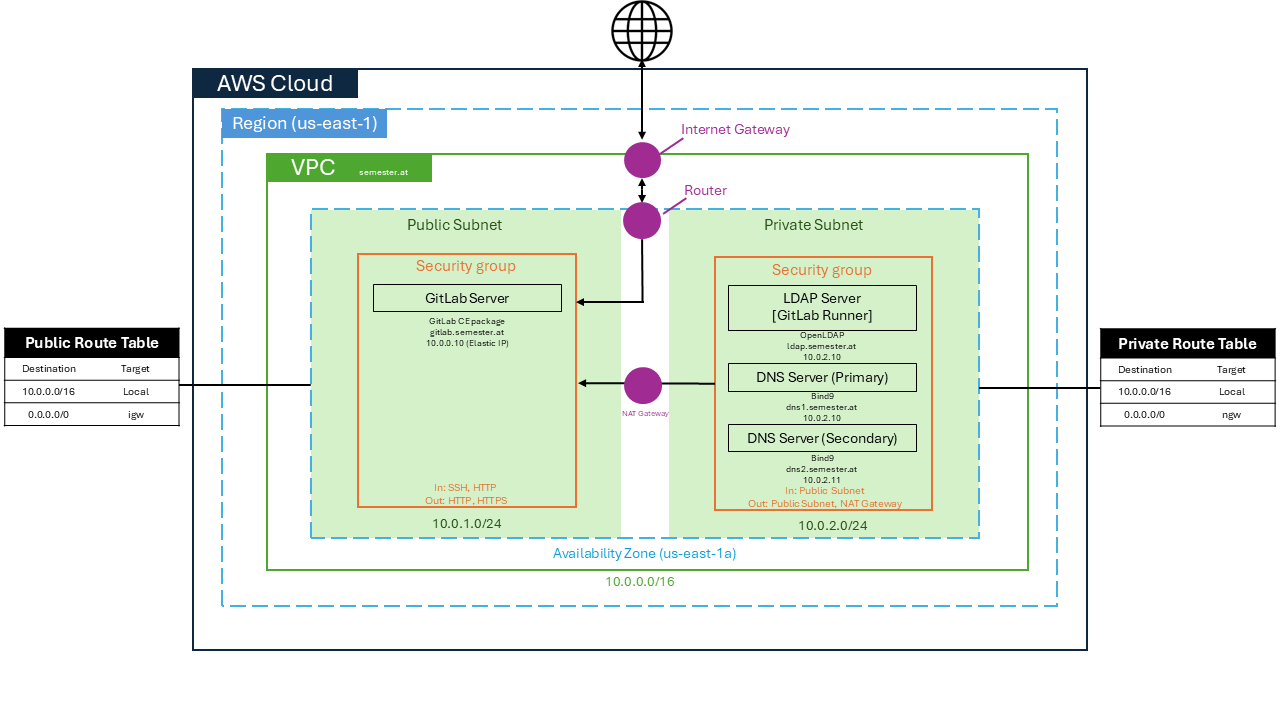
\includegraphics[width=\textwidth]{data/DevOps_Network_Topology.png}
	\caption{Netzwerktopologie der Infrastruktur}
	\label{fig:network_topology}
\end{figure}

\begin{table}[h!]
	\centering
	\begin{tabular}{|l|l|l|l|}
		\hline
		\textbf{Dienst} & \textbf{Subnetztyp}  & \textbf{IP-Adresse} & \textbf{FQDN}      \\ \hline
		Primärer DNS    & Privates Subnetz     & 10.0.2.225          & ns1.semesterDevOps.com   \\ \hline
		Sekundärer DNS  & Privates Subnetz     & 10.0.2.10           & ns2.semesterDevOps.com   \\ \hline
		GitLab Server   & Öffentliches Subnetz & Public              & gitlab.semesterDevOps.com \\ \hline
		LDAP Server     & Privates Subnetz     & 10.0.2.10           & ldap.semesterDevOps.com   \\ \hline
		GitLab-Runner	& Privates Subnetz	   & 10.0.2.184			 & gitlab.semesterDevOps.com \\ \hline
	\end{tabular}
	\caption{Netzwerkdienste und IP-Zuordnung}
\end{table}

\newpage

\section{Geplante Security Groups und Regeln}

\begin{table}[h!]
	\centering
	\begin{tabular}{|l|c|c|c|c|}
		\hline
		\textbf{Inbound SGRs} & \textbf{DNS} & \textbf{LDAP/GitLab-R} & \textbf{GitLab-Server} \\ \hline
		HTTP                  & Nein             & Nein                   & Ja                     \\ \hline
		HTTPS                 & Nein             & Ja                     & Ja                     \\ \hline
		SSH                   & Ja               & Ja                     & Ja                     \\ \hline
		DNS (UDP)             & Ja             & Nein                   & Nein                   \\ \hline
		DNS (TCP)             & Ja             & Nein                   & Nein                   \\ \hline
		LDAP                  & Nein             & Ja                     & Ja                     \\ \hline
		ALL ICMP              & Ja             & Nein                   & Ja                     \\ \hline
	\end{tabular}
	\caption{Eingehende Sicherheitsgruppenregeln (SGRs) für verschiedene Dienste}
	\label{tab:inbound-sgrs}
\end{table}

\begin{table}[h!]
	\centering
	\begin{tabular}{|l|c|c|c|c|}
		\hline
		\textbf{Outbound SGRs} & \textbf{DNS} & \textbf{LDAP/GitLab-R} & \textbf{GitLab-Server} \\ \hline
		HTTP                   & Nein         & Ja                     & Nein                   \\ \hline
		HTTPS                  & Nein         & Ja                     & Nein                   \\ \hline
		SSH                    & Nein         & Ja                     & Nein                   \\ \hline
		DNS (UDP)              & Nein         & Ja                     & Nein                   \\ \hline
		DNS (TCP)              & Nein         & Ja                     & Nein                   \\ \hline
		LDAP                   & Nein         & Ja                     & Ja                     \\ \hline
		ALL ICMP               & Nein         & Ja                     & Nein                   \\ \hline
		ALL Traffic            & Ja           & Nein                   & Ja                     \\ \hline
	\end{tabular}
	\caption{Ausgehende Sicherheitsgruppenregeln (SGRs) für verschiedene Dienste}
	\label{tab:outbound-sgrs}
\end{table}


\newpage
\section{Spezifikationen der eingesetzten Systeme}

\begin{table}[h!]
	\centering
	\resizebox{\textwidth}{!}{
		\begin{tabular}{|l|l|l|l|l|}
			\hline
			\textbf{Server}       & \textbf{OS}   & \textbf{Packages} & \textbf{Version}             & \textbf{Server Instance} \\ \hline
			Primärer DNS Server   & Ubuntu Server & bind9, bind9utils & BIND 9 / Ubuntu 24.04 LTS    & T3.micro                 \\ \hline
			Sekundärer DNS Server & Ubuntu Server & bind9, bind9utils & BIND 9 / Ubuntu 24.04 LTS    & T3.micro                 \\ \hline
			LDAP Server           & Ubuntu Server & slapd, ldap-utils & OpenLDAP 2.6                 & T3.micro                 \\ \hline
			GitLab Runner         & Ubuntu Server & -                 & Ubuntu 24.04 LTS             & T3.micro                 \\ \hline
			GitLab Server         & Ubuntu Server & GitLab CE         & GitLab CE / Ubuntu 24.04 LTS & T2.Large                 \\ \hline
		\end{tabular}
	}
	\caption{Server-Spezifikationen: Betriebssystem, Pakete und Instanztypen}
	\label{tab:server-specs}
\end{table}


\begin{itemize}
	\item \textbf{Betriebssystem}: Ubuntu 24.04 LTS LTS (64-bit)
	\item \textbf{DNS-Server}: BIND 9.x
	\item \textbf{GitLab}: GitLab CE 15.x
	\item \textbf{GitLab Runner}: Version kompatibel mit GitLab CE 15.x
	\item \textbf{LDAP}: OpenLDAP 2.6.x
	\item \textbf{Monitoring}: AWS CloudWatch zur Protokollierung und Überwachung.
\end{itemize}

\newpage

\section{Tests}
\subsection*{DNS Resolution Testing}
\begin{itemize}[leftmargin=1.5cm]
	\item \textbf{Ziel:} Sicherstellen, dass der BIND-Server Domain-Namen korrekt auflöst.
	\item \textbf{Methode:} Verwenden des \texttt{dig}-Befehls, um den DNS-Server nach bekannten Domains abzufragen. Überprüfen der \texttt{A}, \texttt{AAAA}, \texttt{MX} und \texttt{NS} Records:
	      \begin{verbatim}
    dig @<DNS-server> example.com [A, AAAA, MX, NS]
    \end{verbatim}
	\item \textbf{Erwartetes Ergebnis:} Jede Abfrage liefert die richtigen IP-Adressen und Record-Details.
\end{itemize}

\subsection*{Forward and Reverse DNS Lookup}
\begin{itemize}[leftmargin=1.5cm]
	\item \textbf{Ziel:} Überprüfen, dass Vorwärts- und Rückwärts-Abfragen funktionieren.
	\item \textbf{Methode:}
	      \begin{itemize}
		      \item Verwenden von \texttt{dig} für die Vorwärtsabfrage (Domain zu IP):
		            \begin{verbatim}
        dig @<DNS-server> example.com A
        \end{verbatim}
		      \item Verwenden von \texttt{dig -x} für die Rückwärtsabfrage (IP zu Domain):
		            \begin{verbatim}
        dig @<DNS-server> -x [192.0.2.1]
        \end{verbatim}
	      \end{itemize}
	\item \textbf{Erwartetes Ergebnis:} Genaues Mapping zwischen Domain-Namen und IP-Adressen.
\end{itemize}

\subsection*{Zone Transfer Test}
\begin{itemize}[leftmargin=1.5cm]
	\item \textbf{Ziel:} Sicherstellen, dass Zonentransfers zwischen primären und sekundären DNS-Servern funktionieren.
	\item \textbf{Methode:} Einen Zonentransfer mit \texttt{dig AXFR} anstoßen und die Logs auf den Transfer überprüfen:
	      \begin{verbatim}
    dig @<primary-DNS-server> example.com AXFR
    \end{verbatim}
	\item \textbf{Erwartetes Ergebnis:} Zonendaten werden korrekt zwischen primären und sekundären Servern repliziert.
\end{itemize}

\subsection*{DNS Failover Testing}
\begin{itemize}[leftmargin=1.5cm]
	\item \textbf{Ziel:} Die Resilienz und Zuverlässigkeit des DNS-Dienstes unter Ausfallbedingungen bewerten.
	\item \textbf{Methode:}
	      \begin{itemize}
		      \item Einen Ausfall des primären DNS-Servers simulieren.
		      \item Die Antwort des sekundären DNS-Servers überwachen:
		            \begin{verbatim}
        dig @<secondary-DNS-server> example.com A
        \end{verbatim}
		      \item Etwaige Ausfallzeiten während des Übergangs protokollieren.
	      \end{itemize}
	\item \textbf{Erwartetes Ergebnis:} Der sekundäre DNS-Server übernimmt nahtlos mit wenig bis gar keiner Unterbrechung der DNS-Auflösung.
\end{itemize}

\subsection*{Stress Testing}
\begin{itemize}[leftmargin=1.5cm]
	\item \textbf{Ziel:} Die Leistung des Servers unter hoher Last testen.
	\item \textbf{Methode:} Tools wie \texttt{dnsperf} verwenden, um eine hohe Anzahl von DNS-Abfragen zu simulieren:
	      \begin{verbatim}
    dnsperf -s <primary-DNS-IP> -d queries.txt -l 30
    \end{verbatim}
	\item \textbf{Erwartetes Ergebnis:} Der Server bleibt auch unter Last genau und leistungsfähig.
\end{itemize}

subsection*{LDAP-Authentifizierungstest}
\begin{itemize}[label=--]
	\item \textbf{Ziel:} Funktionalität des Authentifizierungssystems überprüfen.
	\item \textbf{Methode:} Benutzeranmeldungen über LDAP versuchen. Tests mit gültigen und ungültigen Anmeldedaten durchführen.
	\item \textbf{Erwartetes Ergebnis:} Anmeldeversuche sollten für gültige Anmeldedaten akzeptiert und für ungültige Anmeldedaten abgelehnt werden.
\end{itemize}

\subsection*{LDAP-Suche und -Filterung}
\begin{itemize}[label=--]
	\item \textbf{Ziel:} Genauigkeit der LDAP-Suche und -Filterung bestätigen.
	\item \textbf{Methode:} Suchen nach bestimmten Benutzergruppen oder Attributen durchführen und Filter testen.
	\item \textbf{Erwartetes Ergebnis:} Für jede Suche und jeden Filter werden die korrekten Daten zurückgegeben.
\end{itemize}

\subsection*{Benutzer- und Gruppenverwaltung}
\begin{itemize}[label=--]
	\item \textbf{Ziel:} Testen der Erstellung und Änderung von Benutzern und Gruppen.
	\item \textbf{Methode:} Gruppen und Benutzer erstellen sowie deren Attribute ändern. Änderungen im LDAP-Verzeichnis überwachen.
	\item \textbf{Erwartetes Ergebnis:} Alle Änderungen werden korrekt im LDAP-Verzeichnis angezeigt.
\end{itemize}

\subsection*{LDAP-Integrationstest}
\begin{itemize}[label=--]
	\item \textbf{Ziel:} Testen, ob die Integration der GitLab-Authentifizierung mit LDAP funktioniert.
	\item \textbf{Methode:} Anmeldungen bei GitLab mit LDAP-Anmeldedaten (verschiedene Rollen) durchführen.
	\item \textbf{Erwartetes Ergebnis:} Benutzeranmeldungen werden mit LDAP-Anmeldedaten akzeptiert.
\end{itemize}

\subsection*{Repository-Operationen}
\begin{itemize}[label=--]
	\item \textbf{Ziel:} Testen, ob Standard-Git-Operationen innerhalb von GitLab funktionieren.
	\item \textbf{Methode:} Neben der Erstellung von Repositories werden Pull-, Push- und Merge-Operationen getestet. Zusätzlich werden Branches erstellt und gelöscht.
	\item \textbf{Erwartetes Ergebnis:} Änderungen entsprechen den erwarteten Ergebnissen der Git-Operationen.
\end{itemize}

\subsection*{CI/CD-Pipeline-Test}
\begin{itemize}[label=--]
	\item \textbf{Ziel:} Funktionalität der CI/CD-Pipeline überprüfen.
	\item \textbf{Methode:} Geänderten Code pushen und die automatische Ausführung der CI/CD-Pipeline beobachten. Erfolg des Builds und der Bereitstellung prüfen.
	\item \textbf{Erwartetes Ergebnis:} Codeänderungen werden automatisch gebaut und fehlerfrei bereitgestellt.
\end{itemize}

\subsection*{Lasttest}
\begin{itemize}[label=--]
	\item \textbf{Ziel:} Leistung von GitLab unter hoher Last bewerten.
	\item \textbf{Methode:} Mehrere Benutzer simulieren, die gleichzeitig Git-Operationen durchführen.
	\item \textbf{Erwartetes Ergebnis:} GitLab hält die Leistungsniveaus auch bei gleichzeitiger Nutzung aufrecht.
\end{itemize}

\newpage

\section{Rollen und Verantwortlichkeiten im Team}

\begin{table}[h!]
	\centering
	\resizebox{\textwidth}{!}{
		\begin{tabular}{|l|l|l|l|}
			\hline
			\textbf{Samuel Hammerschmidt} & \textbf{Lorenz Rentenberger} & \textbf{Nikolas Schodl} & \textbf{Alexander Weidinger} \\ \hline
			LDAP Server                   & DNS Server (CloudWatch)      & GitLab Server           & GitLab Server                \\ \hline
			AWS Cloud Config              & AWS Cloud Config             & AWS Cloud Config        & AWS Cloud Config             \\ \hline
			Tests LDAP                    & Tests DNS                    & Tests GitLab            & Tests GitLab                 \\ \hline
		\end{tabular}
	}
	\caption{Team-Aufgaben und Zuständigkeiten}
	\label{tab:team-responsibilities}
\end{table}


\section{Monitoring}
AWS CloudWatch wird zur Protokollierung und Überwachung genutzt:
\begin{itemize}
	\item Überwachung der CPU-, Speicher- und Netzwerknutzung.
	\item Automatische Alarme bei Ausfällen.
\end{itemize}

\section{VPC erstellen}

Um ein VPC zu erstellen müssen wir zuerst sicherstellen, dass wir in der richtigen Region sind. 
In unserem Fall ist das 'us-east-1'. 
\begin{figure}[H]
	\centering
	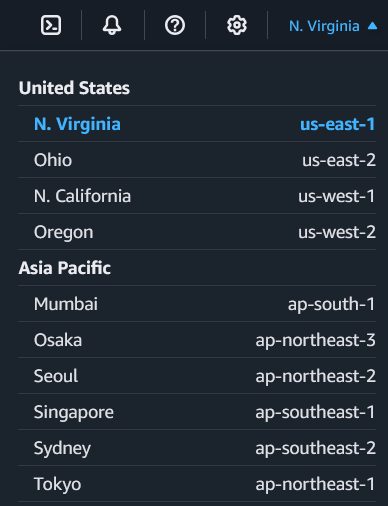
\includegraphics[width=0.5\textwidth]{data/Choose_Region.png}
	\caption{Auswahl der Region}
	\label{fig:Auswahl der Region}
\end{figure}

\section{Creating Subnets}
\subsection{Public Subnet}

Zuerst erstellen wir ein öffenltiches Subnet. 
Wie im Bild unten angeführt, wählen wir den richtigen VPC(10.0.0.0/16) aus
und konfigurieren den privaten CIDR-Block(10.0.1.0/24).
\begin{figure}[H]
	\centering
	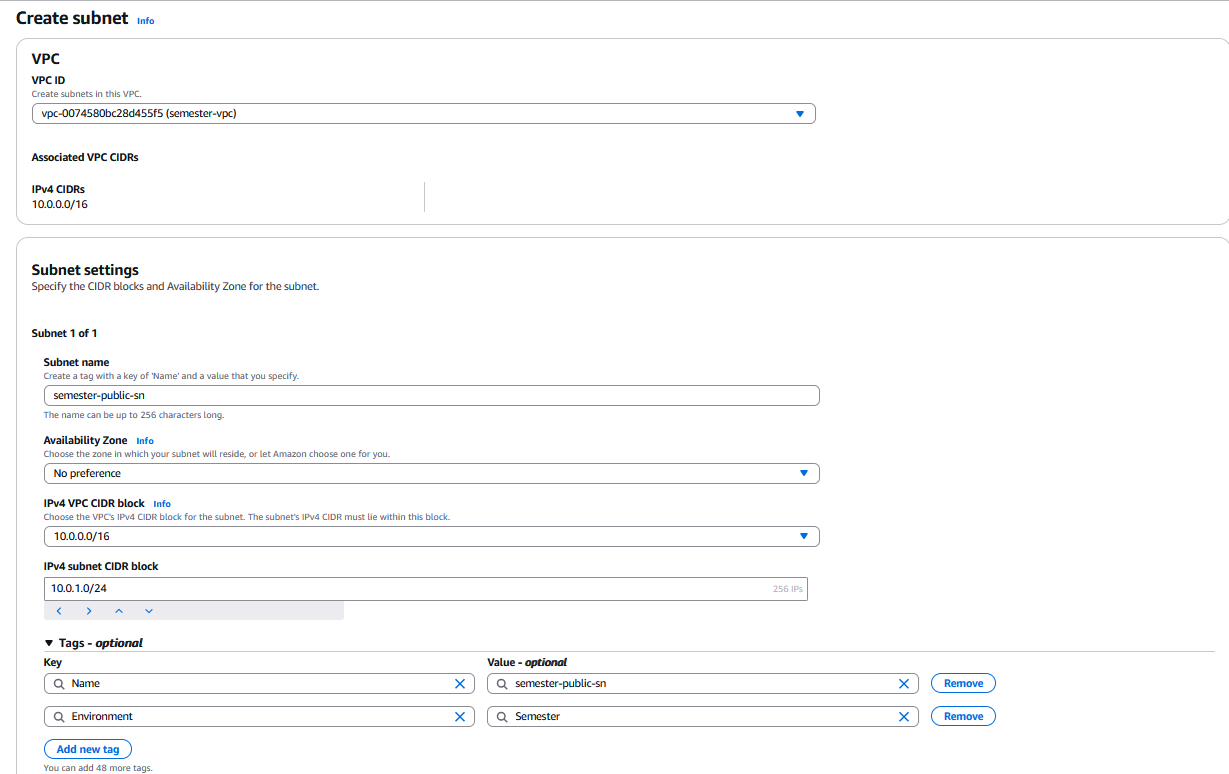
\includegraphics[width=\textwidth]{data/Create_Subnet.png}
	\caption{Erstellung des Public Subnet}
	\label{fig:Erstellung des Public Subnet}
\end{figure}

\subsection{Private Subnet}
Beim Erstellen vom Public Subnet, gehen wir die selbe Schritte durch, 
ändern den CIDR-Block jedoch auf 10.0.2.0/24.

\subsubsection{Enabling Auto-assign IP for Public Subnet}
Wichtig zum Erwähnen ist die Aktivierung der Option 'Enable auto-assign public IPv4 address'. 
Das sorgt dafür, dass jeder neu erstellten EC2 Instanz eine neue IP Adresse zugewiesen wird.
\begin{figure}[H]
	\centering
	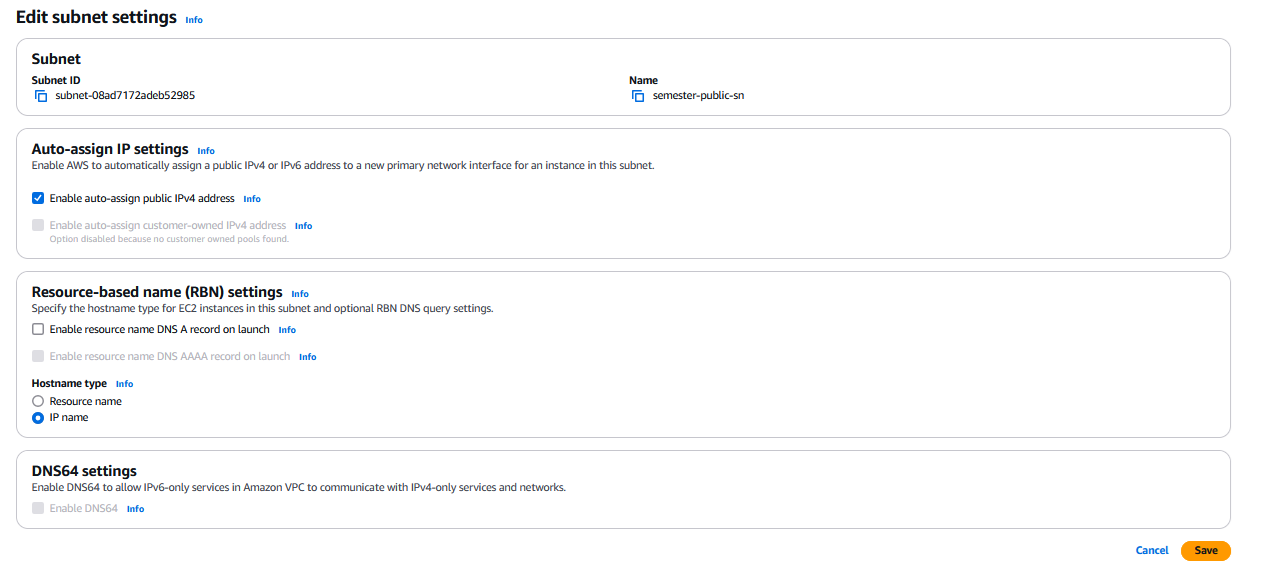
\includegraphics[width=\textwidth]{data/Edit_subnet_enable_ipv4.png}
	\caption{Auto-Assign aktivieren}
	\label{fig:Auto-Assign aktivieren}
\end{figure}



\section{Internet Access}
\subsection{Enabling Internet Access for Public Subnet}
Weiters muss das Public Subnet noch Zugriff auf das Internet bekommen.
Dafür verwenden wir Route-Tables, die wiederum Zugriff auf das Internet Gateway gewähren.

\subsubsection{Internet Gateway}
Zuerst erstellen wir ein Gateway, mit dem Namen 'semester-igw'. 
Dem Gateway geben wir zusätzlich Tags, um später die Suche von diesem zu erleichtern.

\begin{figure}[h!]
	\centering
	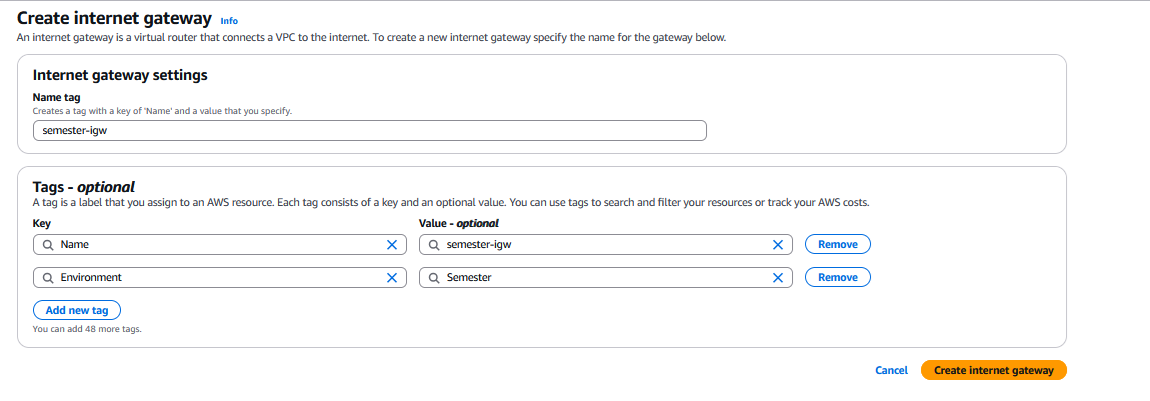
\includegraphics[width=\textwidth]{data/Create_IGW.png}
	\caption{Internet Gateway erstellen}
	\label{fig:Internet Gateway}
\end{figure}

Das Gateway ist erstellt, aber noch keinem VPC zugewiesen. 
Beim Gateway unter 'Actions -> Attach to VPC' fügen wir diesen hinzu.

\begin{figure}[h!]
	\centering
	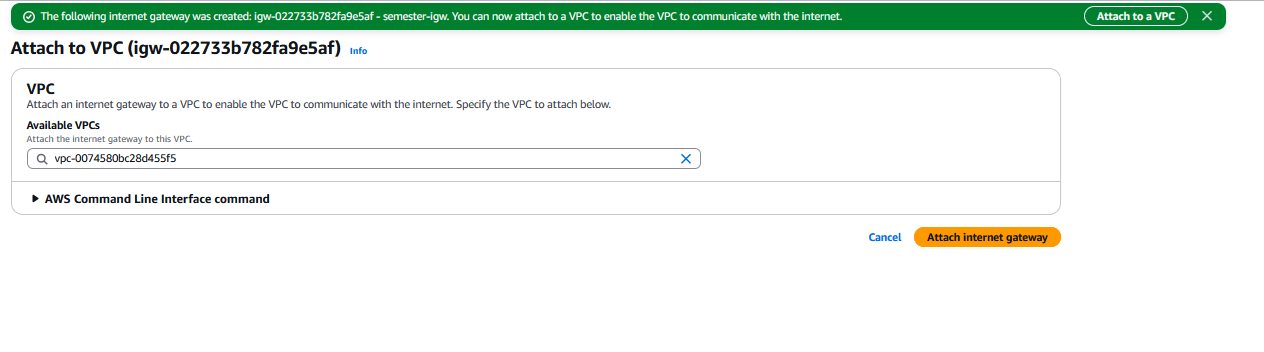
\includegraphics[width=\textwidth]{data/Attach_IGW.png}
	\caption{Internet Gateway einem VPC hinzufügen}
	\label{fig:Attach Internet Gateway}
\end{figure}

\subsubsection{Routing Table}
Jetzt aktualisieren wir die neue Routing Table, damit das Gateway Internetzugriff hat.
In dem Tab 'Route Tables' editieren wir den Table mit dem Namen 'rtb-public-semester'.

\begin{figure}[h!]
	\centering
	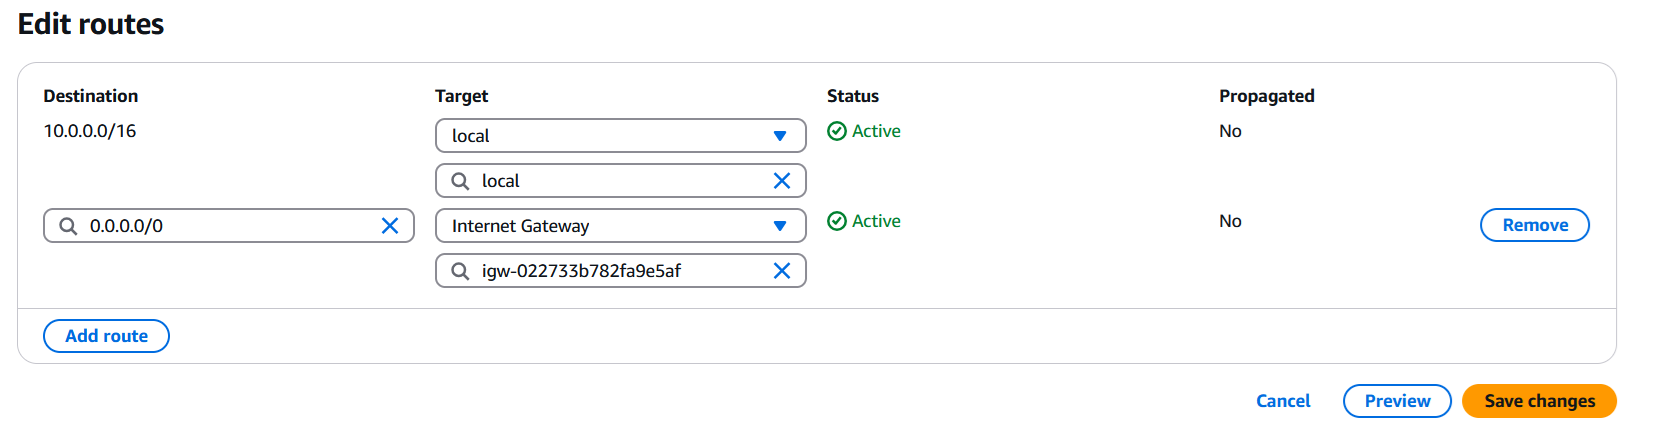
\includegraphics[width=\textwidth]{data/Edit_Routes_Public.png}
	\caption{Routen des Public Route Tables anpassen}
	\label{fig:Attach Routen des Public Route Tables anpassen}
\end{figure}

\subsection{Enabling Internet Access for Private Subnet}
Das private Subnet hat keinen direkten Zugriff, sondern nutzt einen NAT Gateway vom Public Subnet.

\subsubsection{NAT Gateway}
\begin{figure}[h!]
	\centering
	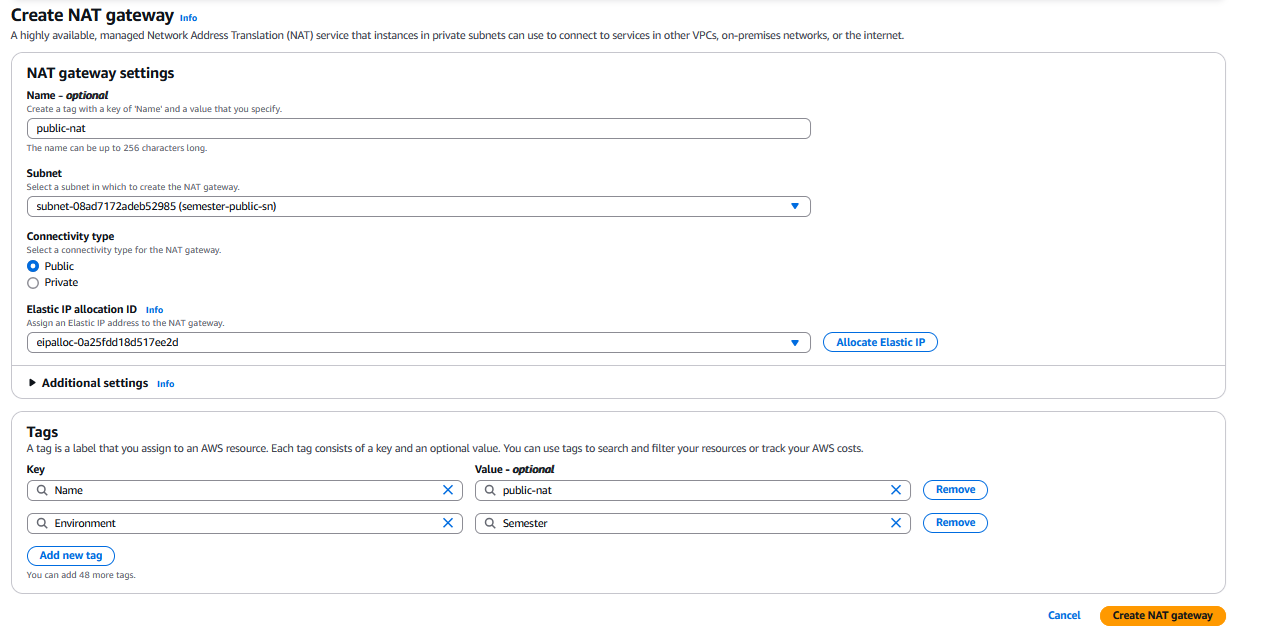
\includegraphics[width=\textwidth]{data/Create_NAT.png}
	\caption{Erstellung des NAT Gateways}
	\label{fig:Erstellung des NAT Gateways}
\end{figure}

\begin{figure}[h!]
	\centering
	\includegraphics[width=\textwidth]{data/Create_Nat2.png}
	\caption{Erstellung des NAT Gateways}
	\label{fig:Erstellung des NAT Gateways}
\end{figure}

\paragraph{Routing Table}
Wie beim Public Subnet, muss man nun die Routing Table aktualisieren, nur für den NAT Gateway anstatt des Internet Gateways.
\begin{figure}[h!]
	\centering
	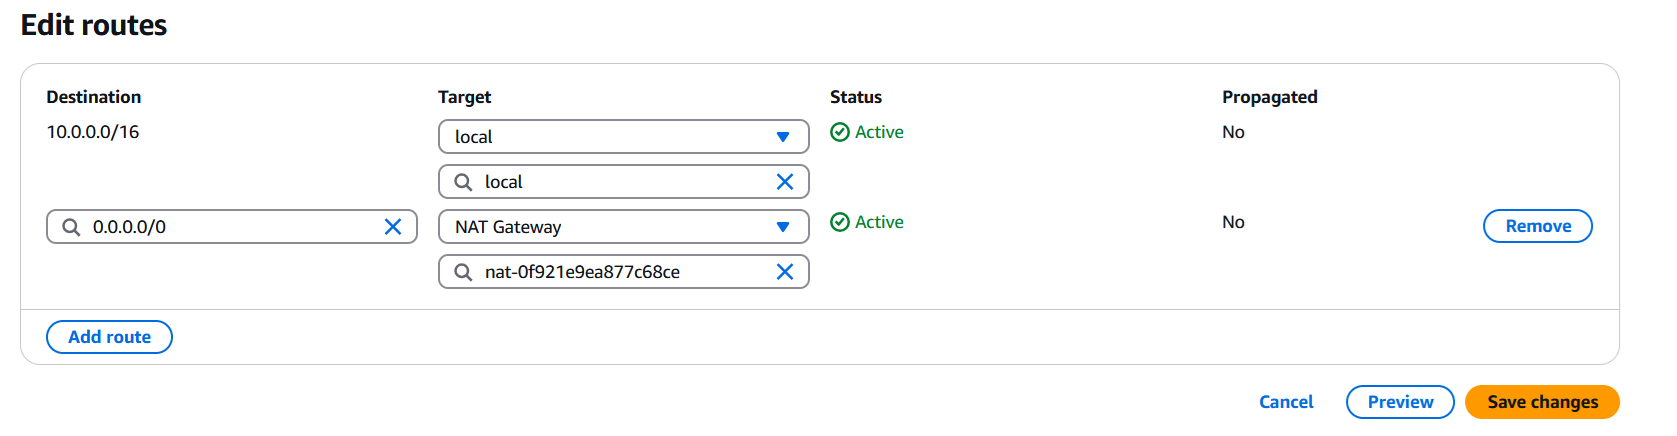
\includegraphics[width=\textwidth]{data/Edit_Routes_Private.png}
	\caption{Routen des Private Route Tables anpassen}
	\label{fig:Attach Routen des Private Route Tables anpassen}
\end{figure}

\newpage

\section{Security Groups}
Für das Projekt haben wir mehrere Security Groups erstellt.
\subsection{Public GitLab}
\begin{table}[h!]
	\centering
	\resizebox{\textwidth}{!}{
		\begin{tabular}{|l|l|l|l|l|}
			\hline
			\textbf{Type}       & \textbf{Internet-Protokoll}   & \textbf{Port} & \textbf{Source}   & \textbf{Desc.}   \\ \hline
			Inbound   	& TCP 	& 80 		& 0.0.0.0/0    	& HTTP                 			\\ \hline
			Inbound 	& TCP 	& 443 		& 0.0.0.0/0    	& HTTPS                			\\ \hline
			Inbound     & TCP 	& 22 		& 0.0.0.0/0     & SSH(GitLab)               	\\ \hline
			Inbound     & TCP 	& 2424      & My IP         & SSH(Admin)                	\\ \hline
			Outbound    & ALL 	& ALL       & 0.0.0.0/0		& Allow all outbound traffic    \\ \hline
		\end{tabular}
	}
	\caption{Security Group: Public GitLab}
	\label{tab:sec-Group-GitLab-Public}
\end{table}

\subsection{Private GitLab}
\begin{table}[h!]
	\centering
	\resizebox{\textwidth}{!}{
		\begin{tabular}{|l|l|l|l|l|}
			\hline
			\textbf{Type}       & \textbf{Internet-Protokoll}   & \textbf{Port} & \textbf{Source}   & \textbf{Desc.}   \\ \hline
			Inbound   	& TCP 	& 80 		& 0.0.0.0/0    	& HTTP                 			\\ \hline
			Inbound 	& TCP 	& 443 		& 0.0.0.0/0    	& HTTPS                			\\ \hline
			Inbound     & TCP 	& 22 		& 0.0.0.0/0     & SSH			               	\\ \hline
			Outbound    & ALL 	& ALL       & 0.0.0.0/0		& Allow all outbound traffic    \\ \hline
		\end{tabular}
	}
	\caption{Security Group: Private GitLab}
	\label{tab:sec-Group-GitLab-Private}
\end{table}


\subsection{DNS}
\begin{table}[H]
	\centering
	\resizebox{\textwidth}{!}{
		\begin{tabular}{|l|l|l|l|l|}
			\hline
			\textbf{Type}       & \textbf{Internet-Protokoll}   & \textbf{Port} & \textbf{Source}   & \textbf{Desc.}   \\ \hline
			Inbound   	& TCP 	& 53 		& 0.0.0.0/0    	& HTTP                 			\\ \hline
			Inbound 	& TCP 	& 53 		& 0.0.0.0/0    	& HTTPS                			\\ \hline
			Inbound     & TCP 	& 22 		& 0.0.0.0/0     & SSH			               	\\ \hline
			Outbound    & ALL 	& ALL       & 0.0.0.0/0		& Allow all outbound traffic    \\ \hline
		\end{tabular}
	}
	\caption{Security Group: DNS}
	\label{tab:sec-Group-DNS}
\end{table}

\subsection{LDAP}
\begin{table}[H]
	\centering
	\resizebox{\textwidth}{!}{
		\begin{tabular}{|l|l|l|l|l|}
			\hline
			\textbf{Type}       & \textbf{Internet-Protokoll}   & \textbf{Port} & \textbf{Source}   & \textbf{Desc.}   \\ \hline
			Inbound   	& TCP 	& 53 		& 0.0.0.0/0    	& HTTP                 			\\ \hline
			Inbound 	& TCP 	& 53 		& 0.0.0.0/0    	& HTTPS                			\\ \hline
			Inbound     & TCP 	& 22 		& 0.0.0.0/0     & SSH			               	\\ \hline
			Outbound    & ALL 	& ALL       & 0.0.0.0/0		& Allow all outbound traffic    \\ \hline
		\end{tabular}
	}
	\caption{Security Group: LDAP}
	\label{tab:sec-Group-LDAP}
\end{table}


\section{Launch Instance}

Die folgenden Screenshots zeigen, wie wir zwei Ubuntu-Instanzen für Primary und Secondary DNS erstellen können.

\begin{figure}[H]
	\centering
	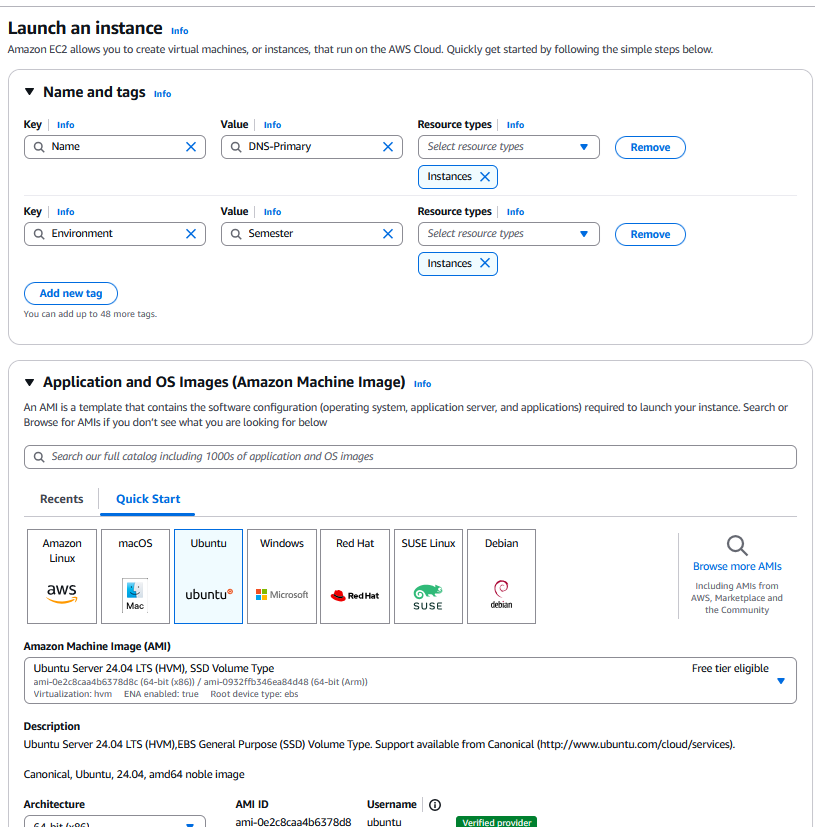
\includegraphics[width=\textwidth]{data/Launch_Instance_DNS_Primary.png}
	\caption{Instanzerstellung vom Primary DNS}
	\label{fig:Instanzecreation vom Primary DNS}
\end{figure}

\begin{figure}[H]
	\centering
	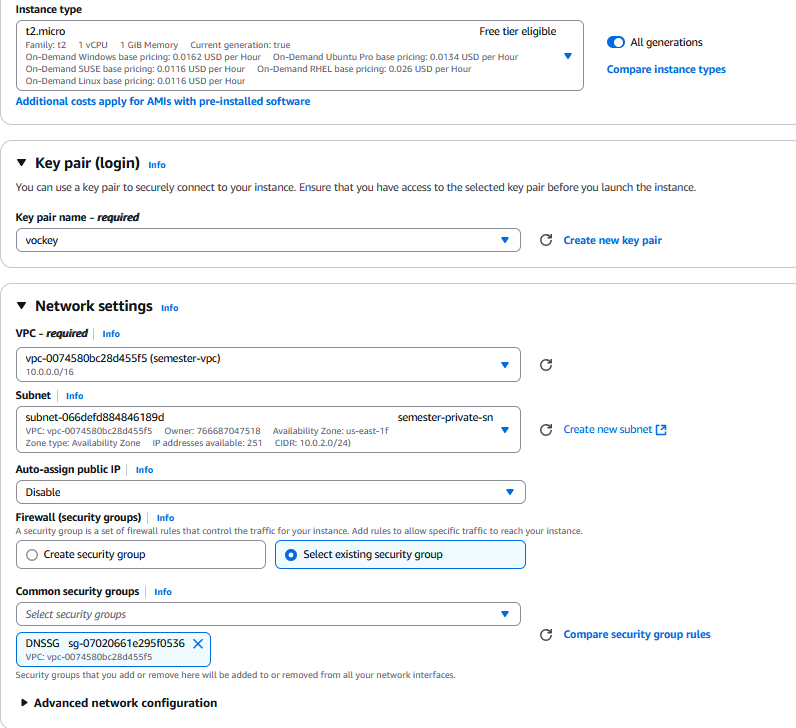
\includegraphics[width=\textwidth]{data/Launch_Instance_DNS_Primary2.png}
	\caption{Instanzerstellung vom Primary DNS}
	\label{fig:Instanzecreation vom Primary DNS2}
\end{figure}

\begin{figure}[H]
	\centering
	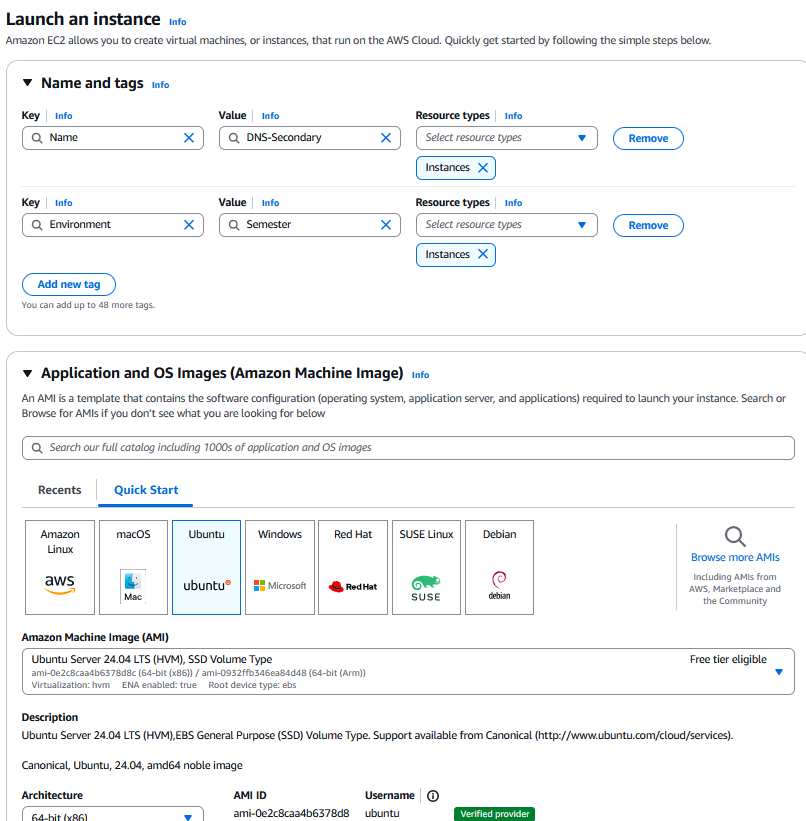
\includegraphics[width=\textwidth]{data/Launch_Instance_DNS_Secondary.png}
	\caption{Instanzerstellung vom Secondary DNS}
	\label{fig:Instanzecreation vom Secondary DNS}
\end{figure}

\begin{figure}[H]
	\centering
	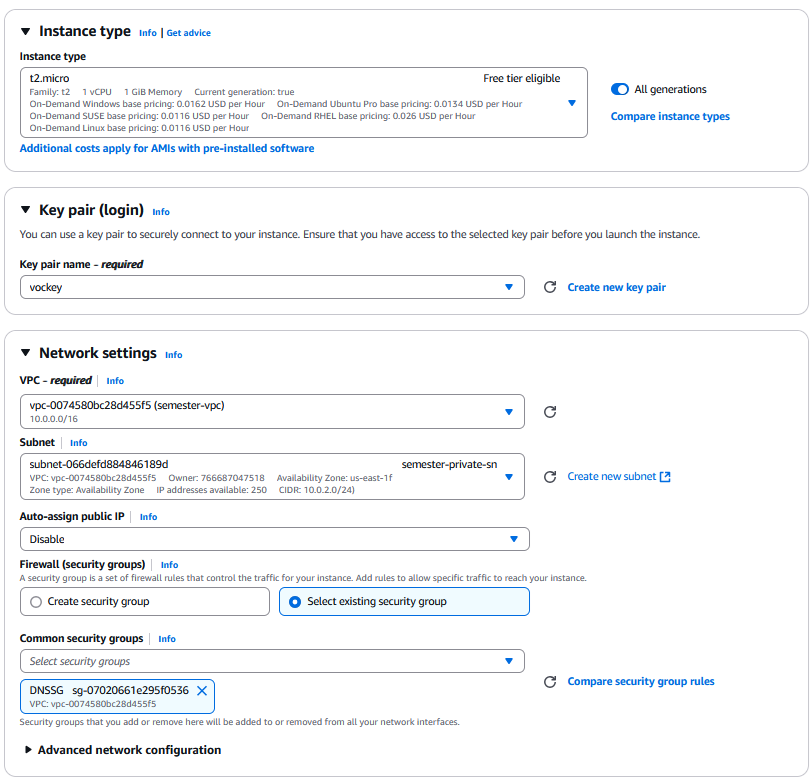
\includegraphics[width=\textwidth]{data/Launch_Instance_DNS_Secondary2.png}
	\caption{Instanzerstellung vom Secondary DNS}
	\label{fig:Instanzecreation vom Secondary DNS2}
\end{figure}

\section{SSH Access zu Server im Private Subnet}
Weil die Server in dem private Subnet keine public IPV4 Adresse haben, können wir nicht auf sie direkt mit SSH zugreifen. 
Wir können um das doch zu erreichen einen Umweg über den GitLab Server nehmen, welcher sich im public Subnet befindet und eine public IPV4 Adresse hat.

\subsection{Setting up SSH Agent Forwarding}
Wir müssen zuerst den SSH Key, den wir von AWS Academy bekommen haben hinzufügen.
\begin{verbatim}
		ssh-add. ~/.ssh/labsuser.pem
\end{verbatim}

Danach ermöglichen wir SSH Agent Forwarding durch Änderung des files \~{} \textit{/.ssh/config}:
\begin{verbatim}
		Host example.com 
		ForwardAgent yes
\end{verbatim}
Nun müssen wir example.com mit der public IPV4 Adresse von GitLab ersetzen. 
Dies muss bei jedem Neustart des GitLab Servers wiederholt werden, weil sich die IP-Adresse bei jedem Start ändert.


\subsection{SSH Zugriff}
Wir können jetzt SSH verwenden um den GitLab Server zu erreichen.
\begin{verbatim}
		ssh ubuntu@93.71.270.50
\end{verbatim}

Und auch um vom GitLab Server zu einem Private Subnet Server springen.
\begin{verbatim}
	ssh ubuntu@10.0.2.225(Private IP des DNS-Primary EC2 Servers)
\end{verbatim}


\subsection{Aktualisieren des Betriebssystems}

Sobald wir auf dem primary DNS Server sind müssen wir zuerst sicherstellen, dass das Betriebssystem auf dem neusesten Stand ist.
Um das zu erreichen führen wir die folgenden Commands aus.
\begin{verbatim}
		sudo apt update && sudo apt upgrade && sudo apt full-upgrade
		sudo reboot
\end{verbatim}


\section{Setup der DNS Server}
Nun konfigurieren wir die beiden DNS Server.
\subsection{Installation von BIND9}
Nachdem wir sichergegangen sind, dass das Betriebssystem auf dem neuesten Stand ist installieren wir BIND9. 
Eine Software Package mit welchem namens resolution machen können. Das erreichen wir mit dem folgenden command:
\begin{verbatim}
		sudo apt install bind9 bind9utils bind9-doc
\end{verbatim}

Wir setzen nun BIND in den IPV4 Modus. Das erreichen wir indem wir das file \textit{/etc/default/named} ändern und -4 am Ende vom OPTIONS Parameter hinzufügen.
\begin{verbatim}
		OPTIONS=“-u bind -4”
\end{verbatim}
Zuletzt starten wir BIND9 neu.
\begin{verbatim}
		sudo systemctl restart bind9
\end{verbatim}



\subsection{Konfiguration des Primary DNS Servers}
Zunächst konfigurieren wir den Primary DNS Server, welcher auf der EC2 Instanz läuft.

\subsubsection{Erstellung der Access Contol List}
Zuerst müssen wir eine ACL(Access Contol List) für den Primary DNS Server erstellen. Dadurch können wir kontrollieren, wer Zugriff auf den Name Server hat.
Die ACL kann in \textit{named.conf.options} geändert werden:
\begin{verbatim}
		sudo nano /etc/bind/named.conf.options
\end{verbatim}


Über dem Options-Block erstellen wir eine neue Access Control List namens trusted.
In dieser benennen wir alle Clients denen wir Zugriff auf den Name Server geben wollen.
\begin{verbatim}
		acl "trusted" {
						10.0.2.184
						10.0.2.225
						10.0.1.246
						10.0.2.10
		};
\end{verbatim}


\subsubsection{Konfiguration der Allgemeine Optionen}
Nun editieren wir den Options Block in dem textit{named.conf.options} File um generelle Einstellungen festzulegen.
\begin{verbatim}
options {
		directory "/var/cache/bind";
		recursion yes; # enables recursive queries
		allow-recursion { trusted; }; # allows recursive queries from "trusted" clients
		listen-on { 10.0.0.0/16; }; # VPC CIDR - listen on private network only
		allow-transfer { none; }; # disable zone transfers by default
		forwarders {
			8.8.8.8;
			8.8.4.4;
		};
		...
};
\end{verbatim}
Wenn der DNS Server eine Anfrage bekommt, welche er nicht selbst beantworten kann, schickt er diese an den unter textit{forwarders} definierten Name Server.


\subsubsection{Konfiguration des “Local” Files}
In der Local File geben wir die Forward- und Reverse-Zonen an, die den Bereich für die Verwaltung und Definition von DNS-Einträgen festlegen.
\begin{verbatim}
		sudo nano /etc/bind/named.conf.local
\end{verbatim}

\subsubsection{Hinzufügen der Forward Zone}
\begin{verbatim}
		zone "semesterDevOps.com" {
		type primary;
		file "/etc/bind/zones/db.semesterDevOps.com"; 
		allow-transfer { 10.0.2.225; };
		};
\end{verbatim}
\textit{type primary} → definiert diesen Server als den Primary Name Server für die Zone. \\
\textit{File} → Pfad zum Zone File \\
\textit{allow-transger} → IP Adressen des sekundären Servers welchem es erlaubt ist, von diesem Server zu transferieren. \\


\subsubsection{Hinzufügen der Reverse Zone für das Public Subnet}
\begin{verbatim}
		zone "1.0.10.in-addr.arpa" {
					type primary;
					file "/etc/bind/zones/db.10.0.1"; # 10.0.1.0/24 Subnet
					allow-transfer { 10.0.2.225; }; # ns2 private IP address - secondary
		};
\end{verbatim}
Um Reverse Lookups zu erlauben, müssen wir die Reverse Zone so konfigurieren, dass wir in der Range unseres Public Subnets sind.


\subsubsection{Hinzufügen der Reverse Zone für das Private Subnet}
\begin{verbatim}
		zone "2.0.10.in-addr.arpa" {
					type primary;
					file "/etc/bind/zones/db.10.0.2"; # 10.0.2.0/24 Subnet
					allow-transfer { 10.0.2.225; }; # ns2 private IP address - secondary
					};
\end{verbatim}
Dasselbe machen wir für das Private Subnet.

\subsubsection{Erstellen des Forward Zone Files}
Die Forward-Zone Datei ist der Ort, an dem wir DNS-Einträge für Forward-DNS-Abfragen definieren. 
Das bedeutet, wenn der DNS eine Namesabfrage erhält, wird er in der Forward-Zonen Datei nachschauen, um die entsprechende private IP-Adresse von host1 zu ermitteln.
Zuerst müssen wir das Directory erstellen. Hier werden wir auch die Forward Zone Files einfügen:
\begin{verbatim}
		sudo mkdir /etc/bind/zones
\end{verbatim}
Jetzt erstellen wir das zone file:
\begin{verbatim}
		sudo nano /etc/bind/zones/db.semesterDevOps.com
\end{verbatim}

\begin{verbatim}
		;
		; BIND data file for local loopback interface
		;
		$TTL 604800
		@ IN SOA ns1.semesterDevOps.com. admin.semesterDevOps.com. (
						3 ; Serial
						604800 ; Refresh
						86400 ; Retry
						2419200 ; Expire
						604800 ) ; Negative Cache TTL
		;

		; name servers - NS records
				IN	NS 	ns1.semesterDevOps.com.
				IN 	NS 	ns2.semesterDevOps.com.

		; name servers - A records
		ns1.semesterDevOps.com. 	IN	A		10.0.2.225
		ns2.semesterDevOps.com. 	IN	A		10.0.2.10

		; 10.0.0.0/16 - A records
		gitlab.semesterDevOps.com. IN 	A 	10.0.1.246
		glrunner.semesterDevOps.com. 	IN 	A 	10.0.2.184
\end{verbatim}


\subsubsection{Erstellen des Reverese Zone Files für das Public Subnet}
Reverse-Zonen Dateien sind der Ort, an dem wir DNS PTR-Einträge für Reverse-DNS-Abfragen definieren. 
Das bedeutet, wenn der DNS eine Abfrage nach einer IP-Adresse erhält, z. B. 10.0.1.77, wird er in der Reverse-Zonen Datei nachschauen, um den entsprechenden FQDN zu ermitteln, z.B. gitlab.semesterDevOps.com in diesem Fall.
Lassen Sie uns die Zonendatei erstellen:

\begin{verbatim}
		sudo nano /etc/bind/zones/db.10.0.1
\end{verbatim}
\begin{verbatim}
		;
		; BIND reverse data file for 10.0.1.0/24
		;
		$TTL 604800
		@ IN SOA ns1.semesterDevOps.com. admin.semesterDevOps.com. (
				2024011201 ; Serial (YYYYMMDDnn)
				604800 ; Refresh
				86400 ; Retry
				2419200 ; Expire
				604800 
		) ; Negative Cache TTL
		;
		; Name servers - NS records
		IN NS ns1.semesterDevOps.com.
		IN NS ns2.semesterDevOps.com.
		; PTR Records
		77 IN PTR gitlab.semesterDevOps.com. ; 10.0.1.246
\end{verbatim}

\begin{itemize}
	\item semesterDevOps.com. oder @ : Wurzel der Zone. Dies gibt an, dass die Zonendatei für die Domain semesterDevOps.com bestimmt ist.
@ ist nur ein Platzhalter, der den Inhalt der \${}ORIGIN-Variable ersetzt.

\item IN SOA: Der Teil „IN“ steht für Internet. SOA ist der Hinweis darauf, dass dies ein Start of Authority-Eintrag ist.

\item ns1.semesterDevOps.com.: Definiert den primären Name Server für diese Domain.

\item admin.semesterDevOps.com.: E-Mail-Adresse des Administrators für diese Zone. Das „@“ wird in der E-Mail-Adresse durch einen Punkt ersetzt.

\item Serial: Seriennummer für die Zone Datei. Jedes Mal, wenn die Zone Datei bearbeitet wird, muss diese Nummer inkrementiert werden, damit die Zonendatei korrekt propagiert wird.
Sekundäre Server prüfen, ob die Seriennummer der Zone auf dem primären Server größer ist als die, die sie auf ihrem System haben. Ist dies der Fall, fordert der sekundäre Server die neue Zonendatei an; wenn nicht, wird weiterhin die ursprüngliche Datei bereitgestellt.

\item Refresh: Aktualisierungsintervall für die Zone. Dies ist der Zeitraum, den der sekundäre Server wartet, bevor er den primären Server auf Änderungen der Zonendatei abfragt.

\item Retry: Wiederholungsintervall für diese Zone. Wenn der sekundäre Server nach Ablauf des Aktualisierungsintervalls keine Verbindung zum primären Server herstellen kann, wartet er diesen Zeitraum und versucht dann erneut, den primären Server abzufragen.

\item Expire: Ablaufzeitraum. Wenn ein sekundärer Name Server den primären Server für diesen Zeitraum nicht kontaktieren konnte, gibt er keine Antworten mehr als autoritative Quelle für diese Zone zurück.

\item Negative Cache TTL: Zeitraum, für den der Name Server einen Namensfehler zwischenspeichert, wenn der angeforderte Name in dieser Datei nicht gefunden werden kann.
\end{itemize}

\newpage

\subsubsection{Erstellen des Reverse Zone Files für das Private Subnet}
Nun das selbe für das Private Subnet.

\begin{verbatim}
sudo nano /etc/bind/zones/db.10.0.2
\end{verbatim}

\begin{verbatim}
		;
		; BIND reverse data file for 10.0.2.0/24
		;
		$TTL 604800
		@ IN SOA semesterDevOps.com. admin.semesterDevOps.com. (
				1 ; Serial 
				604800 ; Refresh
				86400 ; Retry
				2419200 ; Expire
				604800 
		) ; Negative Cache TTL
		;
		; Name servers - NS records
		IN NS ns1.semesterDevOps.com.
		IN NS ns2.semesterDevOps.com.
		; PTR Records
		252 IN PTR ns1.semesterDevOps.com. ; 10.0.2.225
		217 IN PTR ns2.semesterDevOps.com. ; 10.0.2.10
		148 IN PTR glrunner.semesterDevOps.com. ; 10.0.2.184
\end{verbatim}

\paragraph{Überprüfen der BIND Configuration Syntax}
Wir können die Syntax aller named.conf* Files mit dem folgenden Command überprüfen:

\begin{verbatim}
		sudo named-checkconf
\end{verbatim}
Um die Zone Files zu überprüfen helfen uns diese Commands:
\begin{verbatim}
		sudo named-checkzone 1.0.10.in-addr.arpa /etc/bind/zones/db.10.0.1
		sudo named-checkzone 2.0.10.in-addr.arpa /etc/bind/zones/db.10.0.2
\end{verbatim}
Sobald die Syntax überprüft wurde, müssen wir BIND9 neustarten, damit die Änderungen übernommen werden:
\begin{verbatim}
		sudo systemctl restart bind9
\end{verbatim}

\section{Konfiguration des sekundären DNS-Servers}  
Der sekundäre DNS-Server wird alle Einträge des primären DNS-Servers spiegeln 
und alle Anfragen beantworten, wenn der primäre DNS-Server nicht verfügbar ist.  

\subsection{Einrichten der Zugriffskontrollliste und allgemeiner Optionen}  

Sowie der erste DNS, brauch der Zweite ebenfalls eine Access control list.
\begin{verbatim}
	acl "trusted" {
		10.0.2.225
		10.0.2.10
		10.0.1.246
		10.0.2.184
	};

	options {
			directory "/var/cache/bind";
			recursion yes; # enables recursive queries
			allow-recursion { trusted; }; # allows recursive queries from "trusted" clients
			listen-on { 10.0.0.0/16; }; # VPC CIDR - listen on private network only
			allow-transfer { none; }; # disable zone transfers by default
			forwarders {
				8.8.8.8;
				8.8.4.4;
			};
			...
	};
\end{verbatim}


\subsection{Konfigurieren vom Local File}
Die Local Files vom zweiten DNS wird genau so konfiguriert wie vom Ersten. 
Es gibt nur kleine Unterschiede wie die "type": 


\begin{verbatim}
	zone "semesterDevOps.com" {
			type secondary;
			file "/etc/bind/zones/db.semesterDevOps.com"; 
			allow-transfer { 10.0.2.225; };
	};
\end{verbatim}


\begin{verbatim}
	zone "1.0.10.in-addr.arpa" {
			type secondary;
			file "/etc/bind/zones/db.10.0.1"; # 10.0.1.0/24 Subnet
			allow-transfer { 10.0.2.225; }; # ns2 private IP address - secondary
	};
\end{verbatim}


\begin{verbatim}
	zone "2.0.10.in-addr.arpa" {
			type secondary;
			file "/etc/bind/zones/db.10.0.2"; # 10.0.2.0/24 Subnet
			allow-transfer { 10.0.2.225; }; # ns2 private IP address - secondary
	};
\end{verbatim}

Zum Überprüfen der Configation verwenden wir:
\begin{verbatim}
	sudo named-checkconf
\end{verbatim}

Wenn alles funkioniert, dann starten wir BIND9 erneut:
\begin{verbatim}
	sudo systemctl restart bind9
\end{verbatim}



\section{Konfiguration der Server}

Unten dargestellt ist die Konfiguration des DNS-Servers auf dem Public-GitLab-Server. 
Es ist jedoch wichtig zu beachten, dass diese Konfiguration auf allen Servern in der Infrastruktur umgesetzt werden muss. 
Zuerst müssen wir herausfinden, welches Gerät mit unserem privaten Netzwerk verbunden ist:

\begin{verbatim}
	ip address show to 10.0.0.0/16
\end{verbatim}


\subsection{Festlegen der Nameserver}  
In Ubuntu werden alle DNS-Dienste über \texttt{systemd} verwaltet. Der für DNS verantwortliche Dienst heißt \texttt{systemd-resolved} und enthält das Dienstprogramm \texttt{resolvectl}, mit dem einige DNS-Konfigurationen vorgenommen werden können.  

Um die Nameserver für DNS-Abfragen auf unsere eigenen DNS-Nameserver festzulegen, können wir den folgenden Befehl verwenden:  

\begin{verbatim}
resolvectl dns <Interface> 10.0.2.225 10.0.2.10
\end{verbatim}  

Hierbei steht \texttt{<Interface>} für die Netzwerkschnittstelle, zum Beispiel \texttt{eth0}.  
Die IP-Adresse \texttt{10.0.2.225} gehört zum primären DNS-Server, und \texttt{10.0.2.10} ist die IP-Adresse des sekundären DNS-Servers. 






\subsection{Änderungen dauerhaft speichern}
Jedoch speichert dieser Command die Änderungen der Einstellungen nicht persistent. Sie würden zum Beispiel nach einem Reboot verloren gehen. 
Um die Änderungen permanent zu machen müssen wir ein paar config-Files ändern: \newline

\begin{verbatim}
	sudo nano /etc/systemd/resolved.conf
\end{verbatim}

Spezifisch das File \textit{etc/systemd/resolved.conf} möchten wir ändern.
Zunächst müssen wir die folgende Zeile anpassen:


\begin{verbatim}
	[Resolve]
	DNS=10.0.2.225 10.0.2.10
\end{verbatim}

Wieder müssen hier IP Adressen des Primary und Secondary DNS angegeben werden.
Damit die Änderungen eintreten müssen wir den \textit{systemd-resolved service} restarten:

\begin{verbatim}
	sudo systemctl restart systemd-resolved
\end{verbatim}

Gehe sicher, dass \textit{/etc/resolv.conf} mit dem Stub-Resolver von \textit{systemd-resolved} verknüpft ist:

\begin{verbatim}
	sudo ln -sf /run/systemd/resolve/resolv.conf /etc/resolv.conf
\end{verbatim}

Mit dem Folgenden Command kann nun auch überprüft werden, ob das System nun wirklich unseren DNS Server verwendet:

\begin{verbatim}
	sudo resolvectl status
\end{verbatim}

\subsection{Testen der Nameserver}
Wir können überprüfen, ob unsere Nameserver funktionieren, indem wir einige Abfragen durchführen. Wir beginnen mit DNS-Forward-Lookups:

\begin{verbatim}
	nslookup gitlab.semesterDevOps.com
\end{verbatim}

Sobald wir bestätigt haben, dass diese ordnungsgemäß funktionieren, führen wir auch DNS-Reverse-Lookups durch:


\begin{verbatim}
	nslookup glrunner.semesterDevOps.com
\end{verbatim}


Alternativ können wir auch den Befehl dig verwenden, um detailliertere Ausgaben zu erhalten:

\begin{verbatim}
	nslookup 10.0.1.246
\end{verbatim}

\begin{verbatim}
	nslookup 10.0.2.184
\end{verbatim}


\subsection{Überprüfen, ob der sekundäre DNS-Server wie vorgesehen funktioniert}  
Es gibt mehrere Möglichkeiten, um zu testen, ob der sekundäre DNS-Server wie vorgesehen arbeitet:  

\begin{enumerate}  
    \item \textbf{Direkte Abfrage des sekundären DNS-Servers mit \texttt{dig}}  
    \begin{verbatim}
    dig @10.0.2.10 gitlab.semester.DevOps.com
    \end{verbatim}  

    \item \textbf{DNS-Primary-Instanz stoppen und Abfragen testen}  
    Stoppen Sie die EC2-Instanz \texttt{DNS-Primary} und überprüfen Sie, ob DNS-Abfragen mithilfe von \texttt{nslookup} oder \texttt{dig} beantwortet werden können.  

    \item \textbf{Lokalen DNS-Cache auf dem Client deaktivieren}  
    Bearbeiten Sie dazu die Datei \texttt{/etc/systemd/resolved.conf} und fügen Sie die folgende Zeile hinzu:  
    \begin{verbatim}
    Cache=no
    \end{verbatim}  
\end{enumerate} 




\newpage

\section{GitLab}

\subsection{Konfiguration des SSH-Ports}
GitLab erlaubt es Benutzern, über SSH auf Repositories zuzugreifen. Dies führt jedoch zu Konflikten mit dem standardmäßigen SSH-Zugang des Systems. Daher ändern wir den SSH-Port des Systems auf \texttt{2424}, sodass der Port \texttt{22} für GitLab verwendet werden kann.
Diese Konfiguration wurde gewählt, da das Klonen eines Repositories eine häufigere Aufgabe ist als der SSH-Zugriff auf den Server. Durch die Verwendung des Standard-Ports für das Repository-Klonen entfällt die Notwendigkeit, einen benutzerdefinierten Port anzugeben. Für den selteneren SSH-Zugriff muss der alternative Port explizit angegeben werden.
Die Änderung wird in der Datei \texttt{/etc/ssh/sshd\_config} vorgenommen:

\begin{verbatim}
Port = 2424
\end{verbatim}

\subsection{Anpassen der Sicherheitsgruppe auf AWS}
Damit eine Verbindung über den Port \texttt{2424} möglich ist, muss dieser Port in der Sicherheitsgruppe \texttt{PublicGitLabSecurityGroup} freigegeben werden. Beachten Sie, dass bei jedem SSH-Zugriff auf die GitLab-Instanz der alternative Port angegeben werden muss:

\begin{verbatim}
ssh ubuntu@98.80.148.9 -p 2424
\end{verbatim}

\subsection{Installation von GitLab CE mit Docker Compose}

Im Anschluss wird Docker gemäß der \href{https://docs.docker.com/engine/install/ubuntu/}{offiziellen Dokumentation} installiert. Nach erfolgreichem Test mit dem \texttt{hello-world}-Image folgen wir der \href{https://docs.gitlab.com/ee/install/docker/installation.html}{GitLab-Dokumentation} für die Installation.

\subsubsection{Erstellen von Verzeichnissen zur Datenpersistenz}
Gemäß der Dokumentation erstellen wir ein Verzeichnis für Konfigurations-, Log- und Daten-Dateien:

\begin{verbatim}
sudo mkdir -p /srv/gitlab
sudo chown -R ubuntu:ubuntu /srv/gitlab
export GITLAB_HOME=/srv/gitlab
\end{verbatim}

\newpage

\subsubsection{Erstellen des Containers mit Docker Compose}
Wir verwenden Docker Compose, um GitLab zu installieren. Dazu erstellen wir eine Datei \texttt{docker-compose.yml} mit folgendem Inhalt:

\begin{verbatim}
services:
  gitlab:
    image: gitlab/gitlab-ce:latest
    container_name: gitlab
    restart: always
    hostname: 'gitlab.semesterDevOps.com'
    environment:
      GITLAB_OMNIBUS_CONFIG: |
        external_url 'http://98.80.148.9'
    ports:
      - '80:80'
      - '443:443'
      - '22:22'
    volumes:
      - '$GITLAB_HOME/config:/etc/gitlab'
      - '$GITLAB_HOME/logs:/var/log/gitlab'
      - '$GITLAB_HOME/data:/var/opt/gitlab'
    shm_size: '256m'
\end{verbatim}

Die \texttt{external\_url} muss mit der öffentlichen IPv4-Adresse der GitLab-EC2-Instanz aktualisiert werden. Da die IP-Adresse nach jedem Neustart wechselt, ist eine Anpassung der Datei \texttt{docker-compose.yml} nach jedem Neustart notwendig.
Zum Starten des Containers führen wir folgenden Befehl aus:

\begin{verbatim}
docker compose up -d
\end{verbatim}

GitLab ist nach kurzer Zeit unter \texttt{http://98.80.148.9} erreichbar. Der Standard-Benutzername lautet \texttt{root}, das Passwort kann mit folgendem Befehl abgerufen werden:

\begin{verbatim}
docker compose exec -it gitlab cat /etc/gitlab/initial_root_password
\end{verbatim}

\begin{figure}[H]
	\centering
	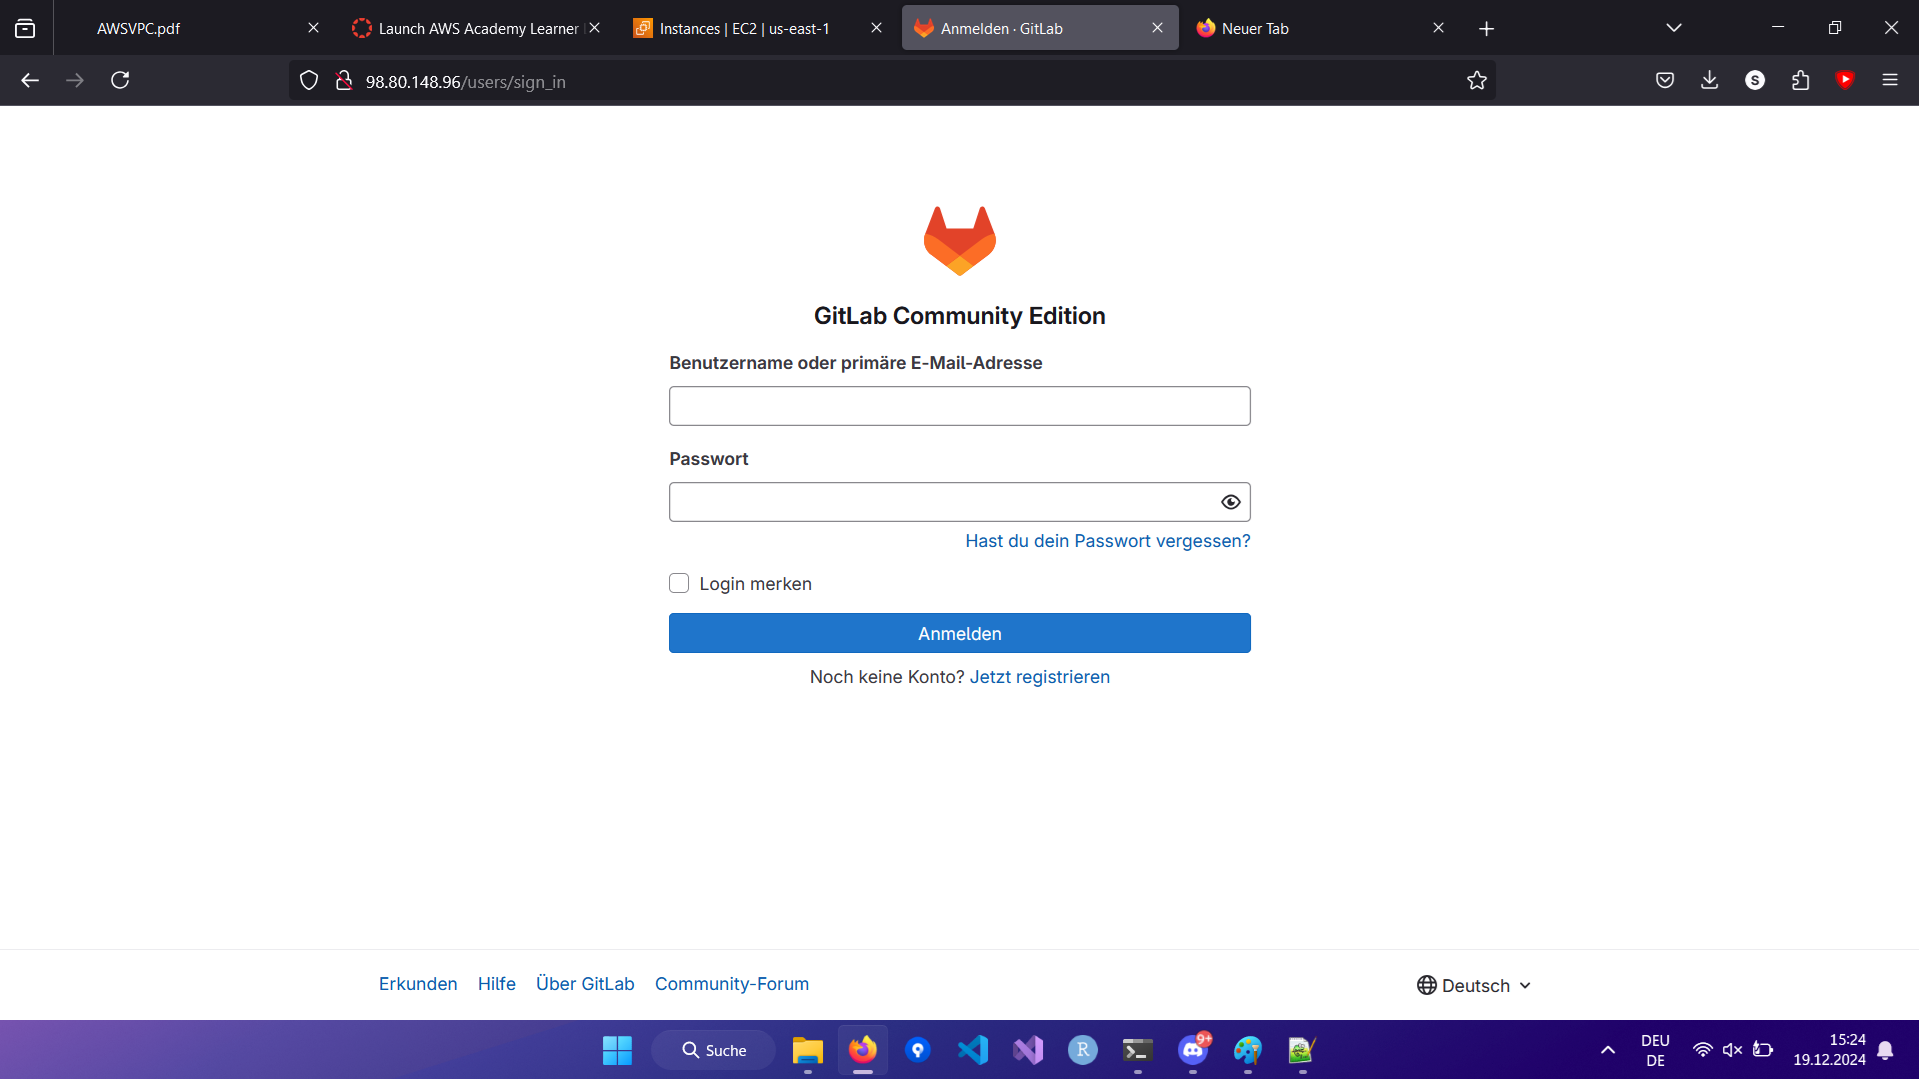
\includegraphics[width=0.8\textwidth]{data/GITLAB_GEHT.png}
	\caption{GitLab läuft}
	\label{fig:GitLab läuft}
\end{figure}

\newpage


\section{GitLab Runner}
Als nächstes installieren wir GitLab Runner auf der GitLab-Runner-EC2-Instanz.  
Wie zuvor verbinden wir uns per SSH mit der Maschine, aktualisieren alle Systempakete, starten die Maschine neu und installieren anschließend Docker gemäß der offiziellen Dokumentation.

\begin{verbatim}
    	docker pull gitlab/gitlab-runner:latest
\end{verbatim}

\subsection{Installation des GitLab Runners mit Docker}
Zuerst laden wir das neueste Docker-Image herunter.  
Anschließend erstellen wir ein neues Docker-Volume, um die Konfiguration auch bei Neustarts des Containers zu behalten.

\begin{verbatim}
		docker volume create gitlab-runner-config
\end{verbatim}

Danach starten wir den GitLab-Runner-Container:

\begin{verbatim}
		docker run -d --name gitlab-runner --restart always \
		-v /var/run/docker.sock:/var/run/docker.sock \
		-v gitlab-runner-config:/etc/gitlab-runner \
		gitlab/gitlab-runner:latest
\end{verbatim}

\subsection{Registrierung des Runners in GitLab}
Um den Runner zu registrieren, folgen wir der \href{https://docs.gitlab.com/runner/register/index.html}{entsprechenden Dokumentation}.  
GitLab-Runner können entweder Projekten, Gruppen oder der gesamten Instanz zugeordnet werden.  
Wir werden unseren Runner mit der gesamten Instanz verknüpfen.

\subsubsection{Erstellen des Runner-Authentifizierungstokens}
Um ein Authentifizierungstoken für den Runner zu erhalten, müssen wir über die GitLab-Weboberfläche einen Instanz-Runner hinzufügen.  
Wie das genau funktioniert, ist in der \href{https://docs.gitlab.com/17.6/ee/ci/runners/runners_scope.html#create-an-instance-runner-with-a-runner-authentication-token}{offiziellen Dokumentation} beschrieben.

\subsubsection{Registrierung des Runners}
Um einen neuen Runner zu registrieren, führen wir folgenden Befehl (auf der GitLab-Runner-EC2-Instanz) aus:

\begin{verbatim}
		docker run --rm -it -v gitlab-runner-config:/etc/gitlab-runner gitlab/gitlab-runner:latest
		register
\end{verbatim}

Nach Ausführung dieses Befehls werden wir aufgefordert, einige Einstellungen vorzunehmen. Diese konfigurieren wir wie folgt:
\begin{itemize}
\item GitLab-Instanz-URL: 
	\\ Hier geben wir \texttt{http://gitlab.SemesterDevOps.com} ein. Diese URL wird von unserem DNS-Server auf den Server aufgelöst, auf dem die GitLab-Instanz läuft.
\item Runner-Authentifizierungstoken: 
	\\ Hier geben wir den \texttt{Token} ein, das in der GitLab-Weboberfläche angezeigt wird.
\item Executor: 
	\\ Wir wählen \texttt{docker}.
\item Standard-Docker-Image: 
	\\ Wir geben \texttt{alpine:latest} ein.
\end{itemize}

\begin{figure}[H]
	\centering
	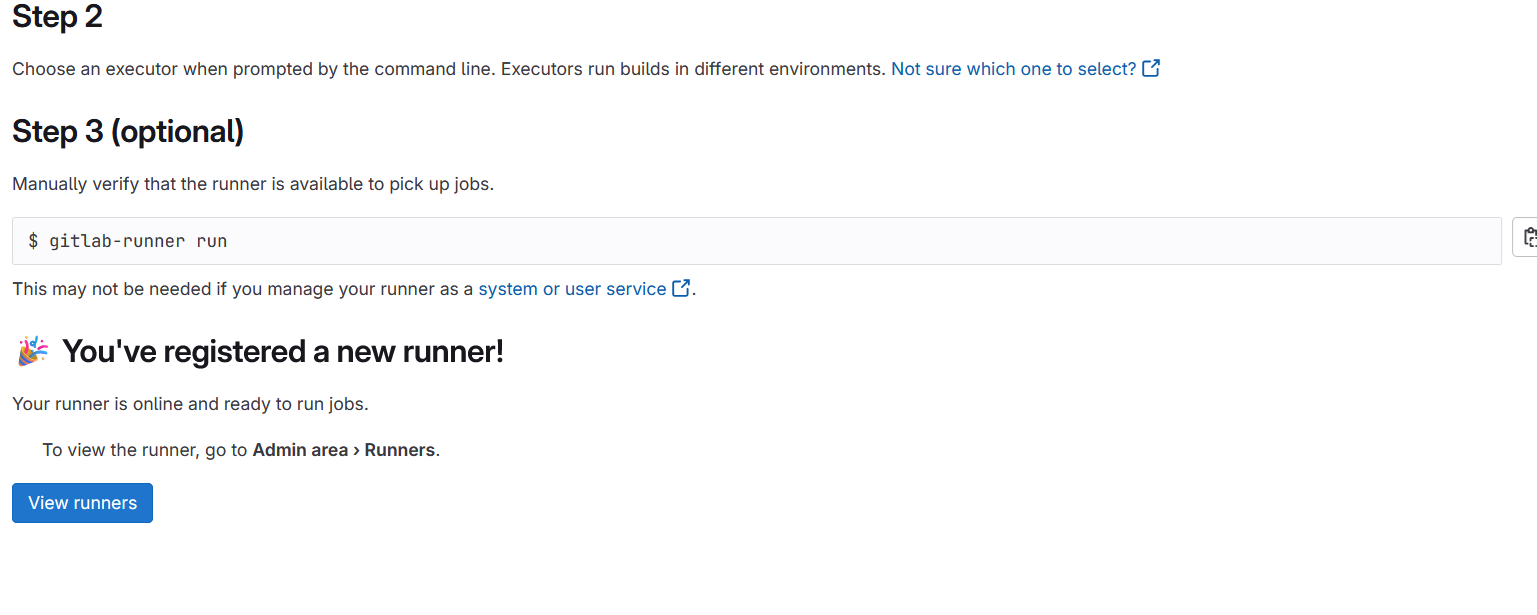
\includegraphics[width=0.8\textwidth]{data/RUNNER_GEHT.png}
	\caption{GitLab Runner registriert}
	\label{fig:GitLab Runner registriert}
\end{figure}
\begin{figure}[H]
	\centering
	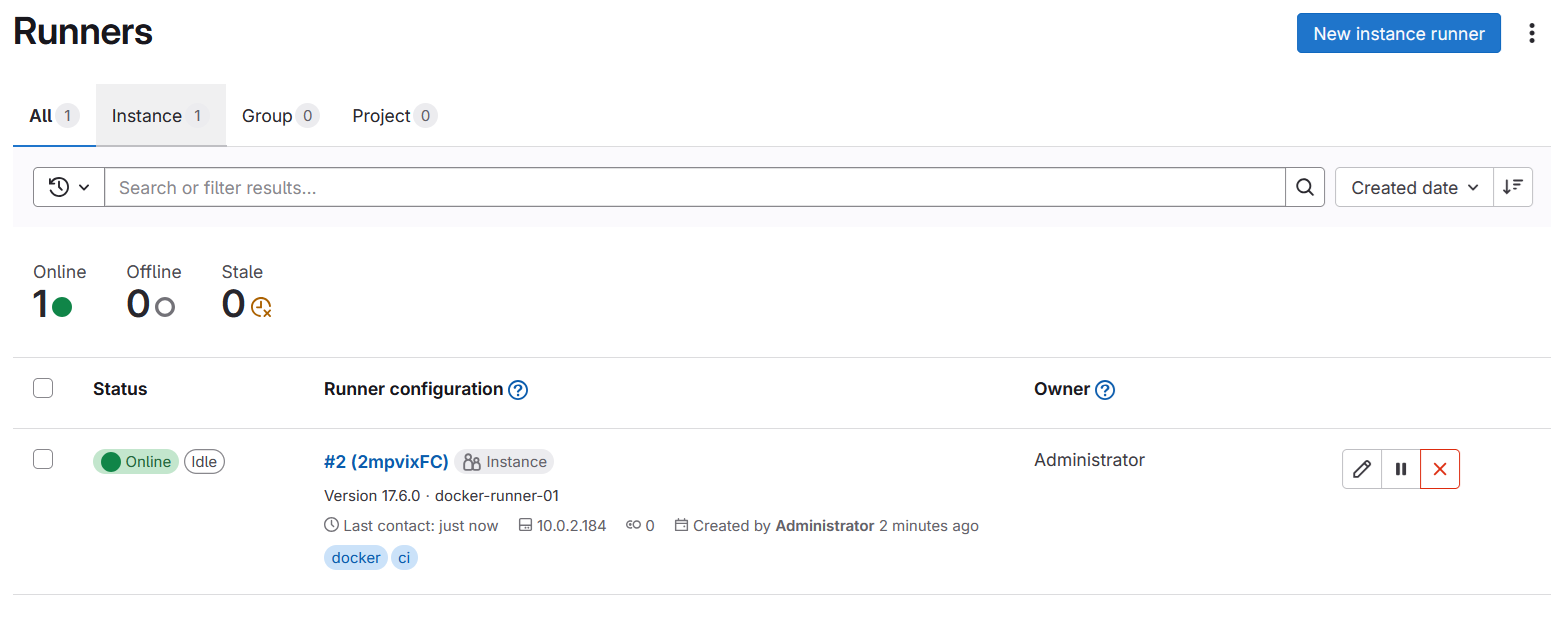
\includegraphics[width=0.8\textwidth]{data/RUNNER_ONLINE.png}
	\caption{GitLab Runner ist Online}
	\label{fig:GitLab Runner ist Online}
\end{figure}


\newpage
\addcontentsline{toc}{section}{Abbildungsverzeichnis}
\listoffigures
\newpage
\addcontentsline{toc}{section}{Tabellenverzeichnis}
\listoftables

\end{document}
